\chapter{Effet Casimir}
    \label{chap-sos}

Dans la section \ref{sec-casimir} nous avons introduit l'effet Casimir comme étant le surplus d'énergie libre causé par le confinement du système, soit 
\begin{align}
    f_c(\beta,L,h) = - k_B T \frac{\partial(L \omega_{ex}(\beta,L,h))}{\partial L}\bigg|_{\beta,L'}
\end{align}
où $\omega_{ex}$ est l'énergie libre en excès dans le système, et prend une forme universelle proche du point critique \cite{casimir-universel}. Cet excès d'énergie libre est dûe à la frustration du système lorsque la longueur de corrélation est du même ordre de grandeur que la taille du système. Dans les systèmes d'interfaces, 
	
%%%%%%%%%%%%%%%%%%%%%%%%%%%%%%%
    \section{Énergie libre d'un système confiné}
%%%%%%%%%%%%%%%%%%%%%%%%%%%%%%%	\textbf{c}
	
\begin{figure}
	\begin{minipage}[t]{0.5\linewidth}
		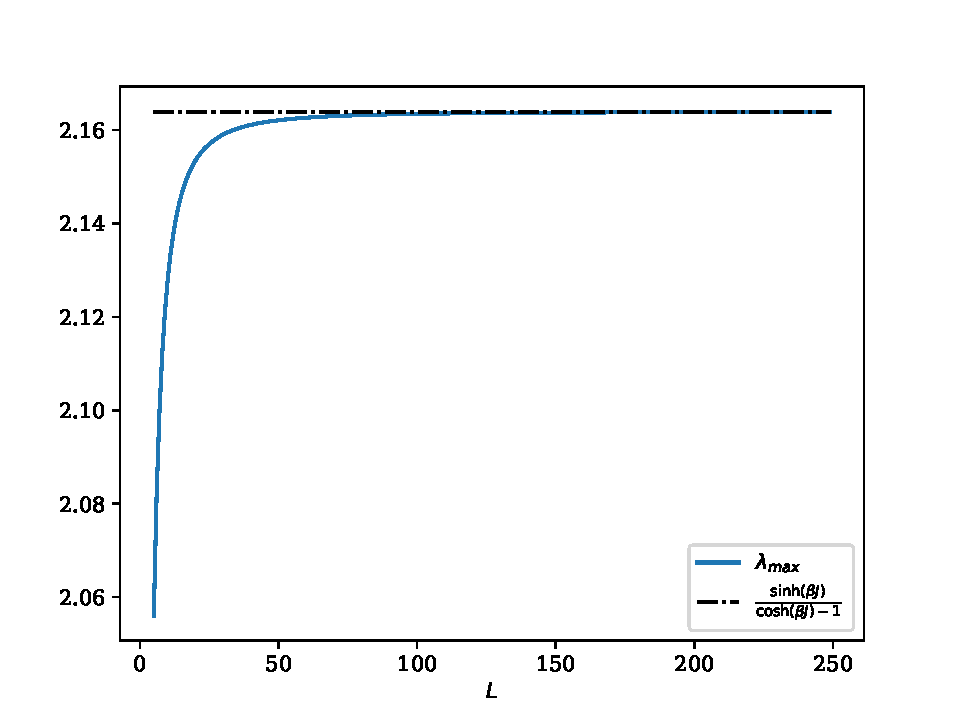
\includegraphics[width=\linewidth]{chap4/freeene-lambda0.pdf}
	\end{minipage}%Cyclin
	\begin{minipage}[t]{0.5\linewidth}
		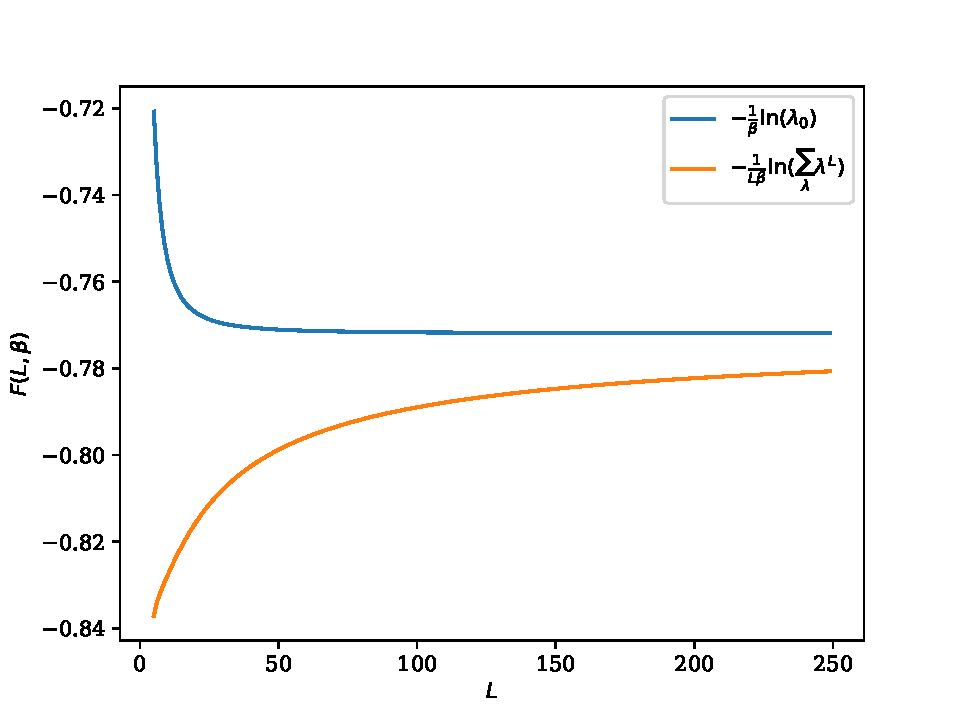
\includegraphics[width=\linewidth]{chap4/freeene-thermo.pdf}
	\end{minipage}
	\caption{Plus grande valeur propre d'une interface libre en fonction de la taille $L$ du système  ayant pour limite \ref{lambda-sos} avec $k=0$ (gauche) ; énergie libre par site calculée via l'approximation de la limite thermodynamique \ref{energie-libre-site} comparé à la vraie fonction de partition \ref{partition-trace-lambda} en fonction de la taille $L$ du système (droite).}
\end{figure}  	

    \subsection{Paramètre d'ordre conservé}
	
    
    \subsection{Intégration sur le paramètre d'ordre}



%%%%%%%%%%%%%%%%%%%%%%%%%%%%%%%
    \section{Conclusion}
%%%%%%%%%%%%%%%%%%%%%%%%%%%%%%%	
	
	
	
	
\begin{comment}	
	\section{Effet du cisaillement}

Dans les expériences, le système est soumis à un cisaillement au niveau de l'interface, ce qui modifie les observables par rapport à l'état d'équilibre. Nous optons ici pour un modèle de cisaillement uniforme dont le sens est défini par $\sgn(i-j)$, $i$ et $j$ étant des sites de hauteurs respectives $h_i$ et $h_j$. 
La différence d'énergie entre un micro-état et le suivant d'une étape de Monte Carlo sous une dynamique de diffusion (Kawasaki) est alors
\begin{align}
	\Delta E = J \sum_i \left[ |h'_i-h'_{i+1}|-|h_i-h_{i+1}| \right] \pm f 
\end{align}
où $h_i'(t) = h_i(t+1)$ - le temps étant discrétisé, $f$ le module de cisaillement et le signe du cisaillement étant pris de manière aléatoire à chaque étape, regardant ainsi si ce mouvement va dans ou contre le sens du flux. 

Pour rappel, à chaque étape on essaie de transférer une particule du site $i$ vers son voisin (gauche ou droit) $j$, ce qui se traduit par $h_i' = h_i-1$ et $h_j' = h_j+1$. 
Pour $f=0$, en remarquant que les valeurs absolues ont les propriétés suivantes
\begin{align}
	|a \pm 1| - |a| = \pm 1 \\
	|a \pm 2| - |a| = {0,\pm 2}
\end{align}
nous voyons facilement l'émergence d'une sélection des énergies possibles entre deux micro-états successifs dans ${-4,-2,0,2,4}$. Ainsi, toutes les transformations diminuant l'énergie totale du système seront toujours acceptées. En augmentant le cisaillement il devient alors possible de refuser des états réduisant l'énergie et d'accepter ceux qui l'augmente. 
Nous nous attendons alors à trois régimes différents :
\begin{itemize}
	\item $f  \less  2 J $ : à faible cisaillement, la symmétrie du système impose les observables à être paire vis-à-vis de $f$, comme le prouve le fit en carré des figures.
	\item $2 J \less f \less 4 J$ : à cisaillement moyen, certains mouvements augmentant la rugosité de l'interface sont toujours acceptés. 
	\item $f > 4 J$ : à haut cisaillement, tous les mouvements augmentant l'entropie du système sont acceptés. Une saturation du système se produit lorsque l'énergie de lien entre les sites devient négligeable face au cisaillement.
\end{itemize}

\end{comment}